\subsection{Fixed Negative Voltage Regulator:}

Following the previous procedure, in this section we analyze two {\bfseries\itshape Fixed Negative Voltage Regulators}. The IC series that we use were the {\bfseries\itshape 79XX}, specifying, the IC {\bfseries\itshape 7905} and the {\bfseries\itshape 7912}. Following the Figure 3.3.0, we assembled 2 very similar circuits but switching between this two IC, in each circuit we connected a voltage source in $V_{in}$ varying it from 3.0 to 16 V in intervals of 1 V:

\begin{figure}[H]
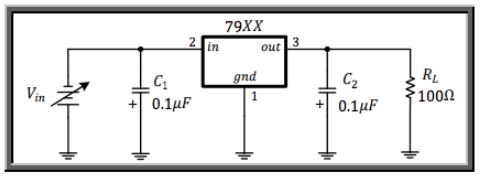
\includegraphics[scale=.6]{d3.png}
\centering \linebreak \linebreak Figure 3.3.0: Fixed negative voltage regulator circuit.
\end{figure}

Once the circuit was assembled, we measure the voltage in the resistor $R_{L}$, and the results were registered in the tables bellow. \hfill \break

{\bfseries\itshape\color{armygreen}{Observation:}} {\itshape\color{armygreen}{For measure the voltage in $R_{L}$ it's necessary to connect a voltmeter in parallel with the resistor.}} \hfill

\begin{multicols}{2}
\begin{tasks}
\task {\bfseries\itshape First Circuit, IC used: 7905:}
\begin{center}
\begin{tabular}[.5cm]{ c c }
\toprule
Source Voltage & Voltage in $R_{L}$ \\
\midrule
3.0 V & -0.56 V \\
\cmidrule{1-2}
4.0 V & -2.3 V \\
\cmidrule{1-2}
5.0 V & -4.2 V \\
\cmidrule{1-2}
6.0 V & -4.9 V \\
\cmidrule{1-2}
7.0 V & -4.9 V \\
\cmidrule{1-2}
8.0 V & -4.9 V \\
\cmidrule{1-2}
9.0 V & -4.9 V \\
\cmidrule{1-2}
10.0 V & -4.9 V \\
\cmidrule{1-2}
11.0 V & -4.9 V \\
\cmidrule{1-2}
12.0 V & -4.9 V \\
\cmidrule{1-2}
13.0 V & -4.9 V \\
\cmidrule{1-2}
14.0 V & -4.9 V \\
\cmidrule{1-2}
15.0 V & -4.9 V \\
\cmidrule{1-2}
16.0 V & -4.9 V \\
\bottomrule
\end{tabular}
\end{center} 

\task {\bfseries\itshape Second Circuit, IC used: 7912:}
\begin{center}
\begin{tabular}[.5cm]{ c c }
\toprule
Source Voltage & Voltage in $R_{L}$ \\
\midrule
3.0 V & -1.4 V \\
\cmidrule{1-2}
4.0 V & -3.3 V \\
\cmidrule{1-2}
5.0 V & -4.2 V \\
\cmidrule{1-2}
6.0 V & -5.3 V \\
\cmidrule{1-2}
7.0 V & -6.2 V \\
\cmidrule{1-2}
8.0 V & -7.2 V \\
\cmidrule{1-2}
9.0 V & -8.2 V \\
\cmidrule{1-2}
10.0 V & -9.2 V \\
\cmidrule{1-2}
11.0 V & -10.2 V \\
\cmidrule{1-2}
12.0 V & -11.2 V \\
\cmidrule{1-2}
13.0 V & -11.9 V \\
\cmidrule{1-2}
14.0 V & -11.9 V \\
\cmidrule{1-2}
15.0 V & -11.9 V \\
\cmidrule{1-2}
16.0 V & -11.9 V \\
\bottomrule
\end{tabular}
\end{center} 
\end{tasks}
\end{multicols} 

\pagebreak